\chapter{Concepts and Technologies}
\label{cha:concepts}

\section{Front-end}
\label{cha:concepts:sec:frontend}

\subsection{Typescript}
`` A super-set of JavaScript that compiles to plain JavaScript ''~\cite{tswebsite}, Typescript is a language maintained by Microsoft and developed by \textit{Anders Hejlsberg} in 2012 with the goal of improving the quality and manageability of JavaScript code bases with features such as static typing and object-orientated qualities~\cite{tsrevealed}. Ultimately, Typescript must be compiled to JavaScript before being executed, for compatibility reasons, the default JavaScript target is version ES3 but newer back-ends are also available.

\subsection{HTML}
The \gls{HTML}, the `` World Wide Web's core markup language ''~\cite{html} is a declarative language through which the vast majority of online content is structured, shared and accessed. It is a specification of elements that can be used to structure the content of web pages, such as headings, images, link to other documents, buttons and many others~\cite{htmlcss}.

\subsection{CSS}
\gls{CSS} is another declarative language that pairs with HTML. It's purpose is to describe how the elements present in a web page are presented.
Some of the definitions handle colors, fonts, element arranging, visibility, interaction and many others~\cite{htmlcss}.

\subsection{SASS}
\gls{SASS} is a augmentation of CSS with features that are similar to a object-oriented languages, with loops, variables, functions and rule nesting ~\cite{sass}. SASS files need to be compiled into plain CSS before deployment, there are many of such compilers, some re-generate CSS files upon file  changes.

\subsection{Angular}
Front-end web framework developed as a side project at Google that proved itself as a valuable tool for modern application development. The core idea is that \gls{HTML} faults when it comes to declare dynamic content~\cite{angularjs}, therefore a new middle-ware is introduced between the rendered page and the underling code so that all the elements and events in the \gls{HTML} document are captured and made available to it's components. Such binding goes both ways, so if the state of the underling code changes, the document is re-rendered to reflect the new state.

The first version of Angular is now called AngularJs and can be included in a \gls{HTML} document just like any other JavaScript library. This version proved it's value but was considered confusing and some times, slow. Since then it entered \gls{LTS} stage and no features are added. Angular version 2 and up is a Typescript re-write that includes some new features that aid in the architecture and development of scalable and reusable code, namely, the introduction of Components, Router, Ahead-of-Time compilation and Observables~\cite{angular}.

\todo{Router}
\todo{Components}
\todo{Template}
\todo{angular cli}

\subsection{Angular Material}
Material Design is a set of guidelines and principles made by Google for designing \gls{UI} that aims to bring natural and consistent interactions between users and computers. The guiding principle is based on paper and ink but it is not limited to what they can do in the physical world~\cite{materialdesign}.

Angular Material~\cite{angularmaterial} is the implementation made by Google of components like buttons, text input and separators that follow the Material Design guidelines to be used by Angular applications, providing a consistent look across devices.

\subsection{Sb-Admin-Material}
% introduction
To accelerate the development speed and have faster working prototypes, many web-based projects begin form a ready-made template. This saves time by keeping developers from re-writing common pieces of code commonly referred as ``boilerplate''.

SB Angular Material is a re-write of the famous SB Admin template~\cite{angulartemplate}, a free and open source template developed by Start Bootstrap~\cite{sbadmin} in Angular using components developed in the previously discussed Angular Material project.

As the name implies this template tries to assess the need for an administrator panel, and in doing so it provides a few ready-made components, to name a few, a login component as seen in figure \ref{fig:login}; the main screen with a top and a collapsible side navigation components, seen in figure \ref{fig:dash} and \ref{fig:visible}. This template already encompass some amount of responsive design by toggling the ability of said side navigational panel to be collapsed depending on the user's screen width.

% connection
In the following subsection this template's folder structure will be explained so that one can understand where what are the main parts in which it can be extended to fit any particular project.

\begin{figure}
  \centering
  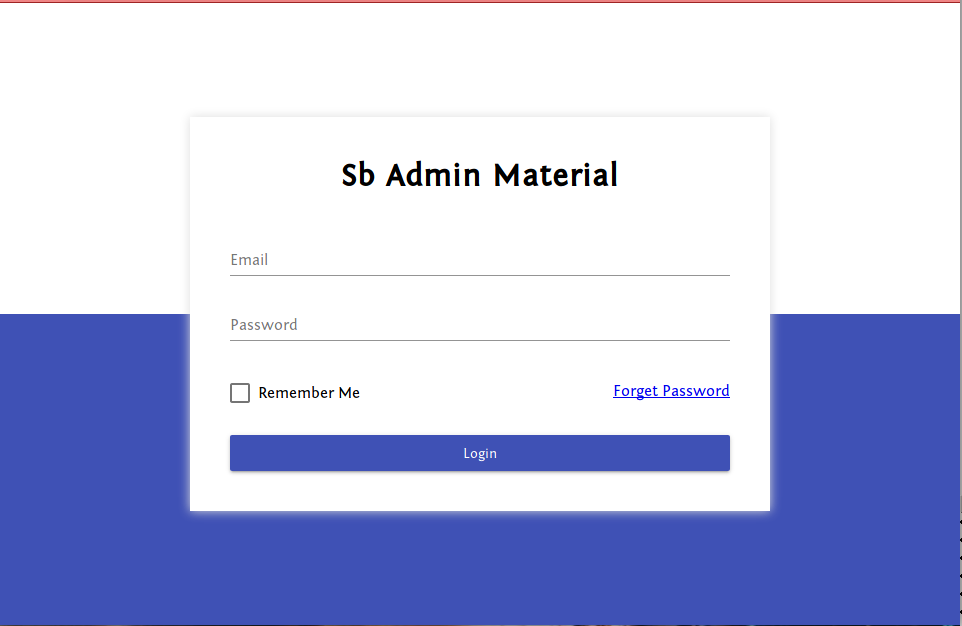
\includegraphics[width=.5\textwidth]{images/sbadmin/login}
  \caption{Login Screen}
  \label{fig:login}
\end{figure}
\begin{figure}
  \centering
  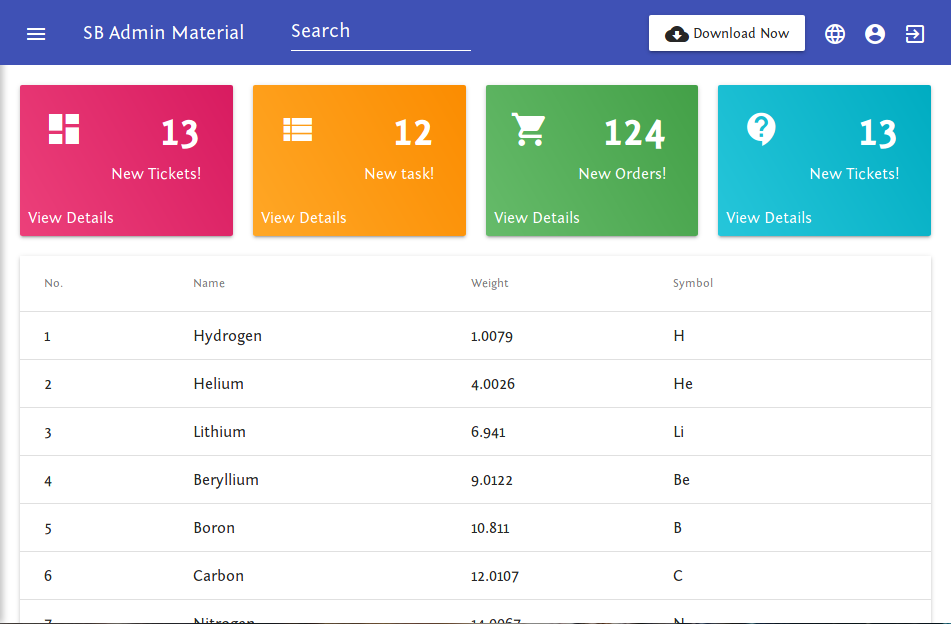
\includegraphics[width=.5\textwidth]{images/sbadmin/collapsed}
  \caption{Dashboard with collapsed side menu}
  \label{fig:dash}
\end{figure}
\begin{figure}
  \centering
  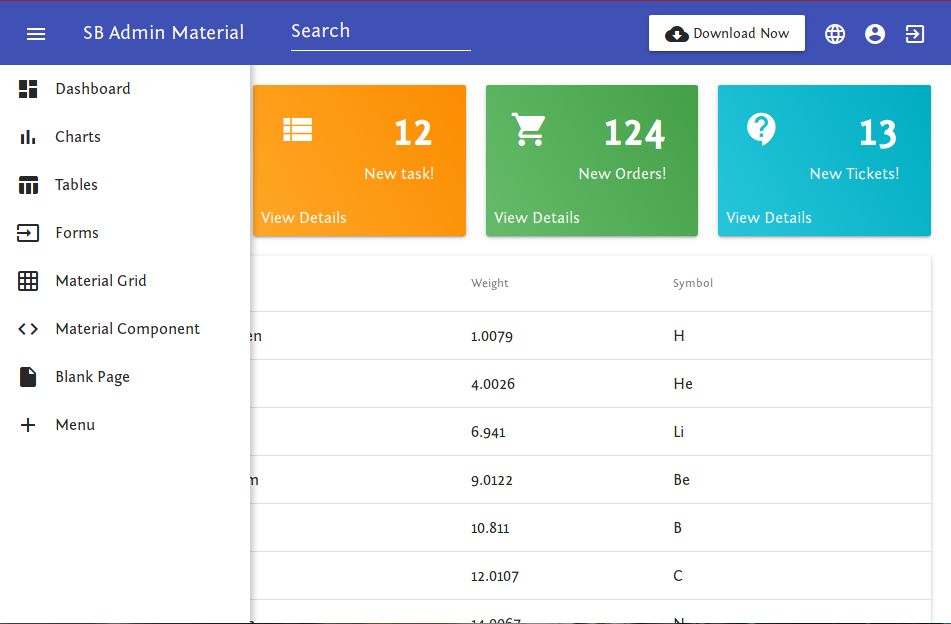
\includegraphics[width=.5\textwidth]{images/sbadmin/visible}
  \caption{Dashboard with visible side menu}
  \label{fig:visible}
\end{figure}

\subsubsection{Project Structure}
% introduction
SB Admin Angular was written with the intention of being modified and extended by other developers. Because the team did not express any guidelines towards how it should be further developed, it is important to give an overview of the current project structure so that the changes made to accommodate the topic of this project are better understood.

\begin{itemize}
\item \textbf{root} This item is not a folder but the root of the project. In here there are configurations for code linter, JavaScript dependency descriptor and the license statement.
\item \textbf{dist} Once the project is built for deployment, this directory will hold all the assets and optimized code ready for production, including the main \texttt{index.html} file that bootstraps the whole project.
\item \textbf{e2e} This holds the source code for End-to-End test cases, hence the name.
\item \textbf{src} This is the heart of this template, a directory that holds all the structure, content and behavior needed per application. \leavevmode
  \begin{itemize}
  \item \textbf{app} The Angular entry-point and application wide router module. \leavevmode
    \begin{itemize}
    \item \textbf{layout} All the components used to compose the navigational elements and menus and their subsequent pages plus some example pages. \leavevmode
      \begin{itemize}
      \item \textbf{black-page} A inaccessible component that does nothing, probably unfinished.
      \item \textbf{blank-page} An example component that is white.
      \item \textbf{charts} A component that display chart capabilities of the integrated JavaScript module chartjs\footnote{Available at https://www.chartjs.org/}.
          \item \textbf{components} Omnipresent page elements such as the Topbar and the collapsible Sidebar.\leavevmode
        \begin{itemize}
        \item \textbf{topnav} The blue navigation top bar as seen on Figure \ref{fig:dash}.
        \item \textbf{sidebar} The Menu on the left side of the screen as seen on Figure \ref{fig:visible}.
        \end{itemize}
      \item \textbf{dashboard} The page in which the user is redirected after logging in.
      \item \textbf{forms} Demonstration of the many different input methods such as Auto Complete text input, Date picker, Text Area and others.
      \item \textbf{grid} A demo of the available page subdivisions.
      \item \textbf{material-components} An example page displaying the main components of Angular Material such as buttons, Dialog and Notifications.
      \item \textbf{nav} Unused component, deprecated by the side bar component.
      \item \textbf{tables} A example component displaying Angular Material's table mechanisms.
      \end{itemize}

    \item \textbf{login} This is the Login component as see on Figure \ref{fig:login}
    \item \textbf{shared} Code that can be used in a application wide manner so that higher abstractions and code reuse can be achieved.
    \end{itemize}
  \item \textbf{assets} Static content directory. Images, fonts, and i18n translations.
  \item \textbf{environments} Depending on how the project is run, either in development or in production mode, a the respective configuration file that holds environment constants is used, allowing developers to use the same reference name throughout the code base no matter the environment.
  \item \textbf{styles} \gls{SASS} files that define the look and feel.
  \end{itemize}
\end{itemize}

% connection
After this overview, it is interesting to note the following:
\begin{itemize}
\item The Layout folder hosts, for the most part, Components and Modules that are listed in the sidebar.\item There are some unused components that were probably left over from design changes and were not deleted, which is the case of black-page and the nav component.
\item There are many examples that proved as a handy reference during development, namely the forms and material-components.
\end{itemize}

\section{Back-end}
\label{cha:concepts:sec:backend}

\subsection{Java}
% introduction
Given how ubiquitous it is, there is not much to be said. Java is a Object-Oriented programming language firstly developed by James Gosling at Sun Microsystems, it is statically and explicitly typed and gets compiled to a machine-independent byte code that is then interpreted by the \gls{JVM}~\cite{java}.

Because of it's high adoption, many concepts were developed to accommodate it's deficiencies and improve the development cycle. In fact, because of the recurring solutions for recurring situations in software design, a group of skilled professionals got together to discuss and write a book entitled ``Design Patterns: Elements of Reusable Object-Oriented Software''~\cite{patterns}, bringing the concept of repeatable ways to some problem.

% connection
This leads to the next topic, View Model, which was used throughout the development of this project to filter the information that is sent to a non-administrator user, removing from the role of filtering sensitive information to the insecure front-end application.

\subsubsection{View Model}
The ViewModel is a piece of a bigger pattern called \gls{MVVM} created by John Gossman to address the scenario in which a model as described in the \gls{MVC} pattern can't be completely mapped to a View~\cite{viewmodel}, therefore it is sensible to specify another model that partially reflects the original model but is able to be completely bound to user interface elements.

During the implementation of this project, the ViewModel pattern was used out of the \gls{MVVM} pattern, however the goal of decoupling code the same. More precisely, some models can not have all of it's attributes serialized back to a View or they expose different attributes depending on the user who is requesting it; ViewModel classes were implemented in such cases.

\subsection{Spring}
% introduction
Developed by Pivotal Software in 2002, the Spring Framework provides most of the ``plumbing'' necessary for fast development and deployment of enterprise Java applications~\cite{springdocs}, some of the main features include: Dependency Injection, a \gls{IoC} mechanism; Spring Data, a set of tools for information access such as \gls{ORM} configurations; Spring Security, a application-wide security mechanisms and configurations.

One of the strongest design philosophies of the Spring Framework is the following:
\begin{displayquote}
``Provide choice at every level. Spring lets you defer design decisions as late as possible. For example, you can switch persistence providers through configuration without changing your code. The same is true for many other infrastructure concerns and integration with third-party \gls{API}s.''~\cite{springdocs}
\end{displayquote}
This leads to a feature-centered development model that is able to quickly deliver prototypes and changes on-demand.

\subsubsection{Dependency Injection}
Conceptually, Dependency Injection is a implementation of the \gls{IoC} principle, abdicating any given class class from managing it's own dependencies; leaving them to a overseer object that knows how to create and inject dependencies to each class\cite{inversion}.

In practical terms, when writing a new class the programmer declare it's dependencies through some mechanism in which the framework is able to reason about. Later in the run-time when a such dependent class is about to be instantiated, it's dependencies are made available and injected into the new instance.

The key idea is that for the most part an application does not need to know which specific class is provided as long as it implements some given interface. It is the Framework's job to choose which class is injected. The programmer, however, is able to tailor the Framework's behavior to their liking.

When using Spring, one can express dependencies by declaring them in the class's constructor or by annotating an attribute using the Autowired annotation\cite{springdi}.

\subsubsection{Data}
When developing a enterprise-level application, often times there is the need of a database management system, an authentication provider and other information-centered services. To address this heterogeneous information storages the Spring Data module was developed that bases itself in a single interface named Repository, through which data is accessed\cite{springdata}.

For the general case the following modules cover the requirements of many applications:
\begin{itemize}
\item Spring Data \gls{JDBC}.
\item Spring Data \gls{JPA}.
\item Spring Data \gls{LDAP}.
\item Spring Data \gls{REST}
\end{itemize}
Note that these libraries are included with the bigger, Spring Data Project.

\subsubsection{\gls{HATEOAS}}
\gls{REST}, according to it's creator:

\begin{displayquote}
  ``REST is a coordinated set of architectural constraints that attempts to minimize latency and network communication, while at the same time maximizing the independence and scalability of component implementations. This is achieved  by  placing  constraints  on  connector  semantics,  where  other  styles have focused on component semantics. REST enables the caching and reuse of interactions, dynamic substitutability of components, and processing of actions by intermediaries, in order to meet the needs of an Internet-scale distributed hypermedia system.''~\cite{fielding}
\end{displayquote}

In other words, this ``new'' architecture expresses requests and responses as the application state itself being transmitted in the client and server approach. There are a few ways in which the state can be communicated and structured, one of which is the subject of this section. 

\gls{HATEOAS} is a response structure that enables a client to discover and navigate related information for that resource\cite{fielding}. Mainly it is able to specify what are the related information, where it is located and how to interact with it. This is accomplished by including some meta-data in the response in which the client can parse, present to the user and issue proper requests.

In the context of Spring Framework, \texttt{CrudRepository} is a interface which can be extended for each class with Entity annotation that needs integration with some kind of persistence mechanism. In it's default implementation there is a \gls{REST} service that is coherent with \gls{HATEOAS}, providing \gls{CRUD} capabilities; indexing as in listing all entries and internal resource linking, which give the ability to retrieve a resource's related resource (think of if like a \gls{RDBMS} table relation).

\subsubsection{Security}
This spring project aims to provide both authentication and authorization mechanisms throughout the application's components, exposing implementable interfaces that enable developers to override necessary parts for their specific needs.

It is important to clarify the distinction between Authentication and Authorization because they have their respective software counterpart that play important roles in Spring Framework.

Authentication, in by definition means ``To prove real or genuine''~\cite{merriamwebster}. In Spring this translates to a custom extension of the \texttt{WebSecurityConfigurerAdapter} abstract class that defines how to verify that a given user exists and is allowed access the resources. There are a few ways to achieve this, two of the most common are: \gls{JDBC} authentication, though which credentials are queried and matched from a \gls{RDBMS} and \gls{LDAP} authentication, that binds to some remote directory for the given user and password pair. Note that it does not define \textit{what} may be accessed by such user, only if the used has access to the system as a whole.

Authorization, ``the act of endorsing, or permitting by some recognized authority''~\cite{merriamwebster}. Similarly to Authentication can also be specified via a custom extension of \texttt{WebSecurityConfigurerAdapter}, and they can co-exist in the same extension. Authorization mechanisms are usually related to some attribute of the current authenticated user, in Spring, the \texttt{GrantedAuthority} interface is the central piece that unifies \textit{what} the user has access to. Authorization points can be defined at the global level by the \texttt{WebSecurityConfigurerAdapter}, at the controller level or at the method level though proper annotations.

\subsubsection{Boot}
Although Spring Framework is a marvelous piece of software for it's malleability and wide range of available features, for a while it was considered a \textit{Configuration Hell} because of it's \gls{XML} configuration that would require a lot of expertise into writing\cite{xmlhell1}\cite{xmlhell2}\cite{xmlhell3}\cite{xmlhell4}\cite{xmlhell5}. In face of this, the Spring Team came up with Spring Boot, a dependency that can be inserted into a project and provides sane, already-configured Spring packages to accelerate development and keep code organized.

\subsection{MariaDB}
A open-source drop-in replacement of MySQL \gls{RDBMS}\cite{mariadb} that started soon after Oracle purchased Sun Microsystems\cite{mariadbfuture}. Developed by the original developers of MySQL it is under active development and a large community\cite{mariadbgit}.

\subsection{LDAP}
\gls{LDAP} in it's core is a protocol defined \gls{IETF}'s \gls{RFC} number 4511\cite{ldaprfc} that defines access to X.500 directory service. Much like  a 

\section{Development}
\subsection{Apache Netbeans}
\subsection{Maven}
\subsection{Lombok}
\subsection{Apache Directory Studio}
\subsection{Visual Studio Code}
\subsection{Docker}
\subsection{Docker-compose}
\subsection{Chinook Database}
\subsection{Angular CLI}
\subsection{Firefox}
\subsubsection{Webpack}
\subsubsection{Debugger}
\subsection{postman}
